\section{Domaine d'application : le réseau local domestique}\label{sec:introduction:digitalhome}
Cette thèse a été développée dans un milieu industriel chez \textit{Orange Labs}. Ainsi, le travail a été motivé par un contexte applicatif posant actuellement de nombreux problèmes en terme de compréhension : le réseau local domestique (ou \textit{Digital Home}).

\begin{figure}[ht]
\centering
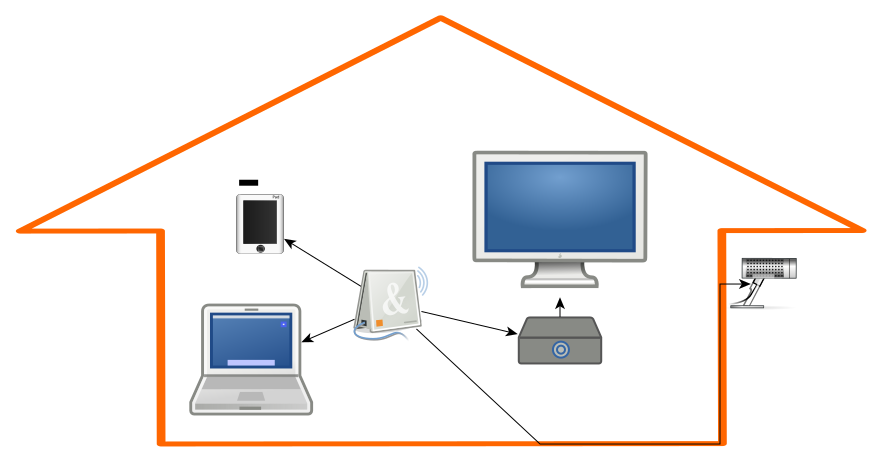
\includegraphics[width=0.7\textwidth]{intro-digitalhome}
\caption{Exemple de réseau local domestique}
\end{figure}

Le réseau local domestique est formé par l'ensemble des appareils d'un utilisateur dans sa maison. Ce réseau est déjà capable de fournir des services tels que le partage de contenus entre un disque dur en réseau (ou \textit{NAS}) sur la télévision ou sur les ordinateurs. L'étape suivante du développement de cette approche est l'introduction de capteurs et d'actuateurs pour effectuer de la domotique. En effet, il devient ainsi possible de créer des automatismes capables de réagir à des événements et d'agir en conséquence. Par exemple : \textit{allumer la lumière si la luminosité n'est pas assez élevée et qu'une personne vient d'entrer dans la pièce.} ou \textit{mettre en veille la télévision si personne n'est actuellement dans la pièce}.

Néanmoins, il n'est pas nécessaire de créer un tel cas d'usage pour soulever des problèmes. En effet, en l'état actuel, les opérateurs qui fournissent des équipements et des services sont bien souvent en difficultés pour dépanner les utilisateurs. Une raison de ce problème est notamment le manque d'informations. Le service après-vente est en effet incapable de connaître la topologie du réseau (utilisation de \textit{wifi} ou courant porteur), la configuration de certains équipements (notamment ceux qu'il ne maîtrise pas) et encore moins l'état de santé des équipements, des liens réseaux ou des services.

Ce cadre applicatif est a fournit des cas d'études et d'expérimentation à cette thèse. Ils réunissent les caractéristiques que nous avons introduit en~\ref{sec:intro:problematique}.
\begin{itemize}
	\item Le réseau domestique est composé de dispositifs hétérogènes.
	\item Les paramètres de configuration et d'autres données accessibles via des services spécifiques sont des données persistantes. Il est possible de récupérer des données de métriques pour mesurer la santé du réseau. Les deux sont nécessaires pour établir une observation unifié.
	\item Chaque équipement fournit ses propres données sous des schémas que nous ne maîtrisons pas.
	\item Certains équipements sont limités en terme de capacités de traitement.
\end{itemize}

En conclusion, nous proposons de développer un système d'observation applicable sur tout système. Nous validerons notre approche par son application sur la compréhension du réseau local domestique. Ceci pourra être utilisé pour aider les diagnostiques fait au service après-vente. Nous présentons maintenant notre approche et les contributions scientifiques de cette thèse.